\documentclass{article}

\usepackage[a4paper]{geometry}
\usepackage[ngerman]{babel}
\usepackage[utf8]{inputenc}
\usepackage[T1]{fontenc}
\usepackage{tabularx}
\usepackage{graphicx}
\usepackage{fancyhdr}
\usepackage{pdfpages}

\graphicspath{{./images/}}

\pagestyle{fancyplain}
\fancyhf{}
\lhead{\fancyplain{}{Mara Schulke} }
\rhead{\fancyplain{}{\today}}
\cfoot{\fancyplain{}{\thepage}}

\begin{document}

\begin{titlepage}
	\begin{flushleft}
		TH Brandenburg \\
		Online Studiengang Medieninformatik \\
		Fachbereich Informatik und Medien \\
		Mensch-Computer-Interaktion \\
		Prof. Dr. Martin Christof Kindsmüller
	\end{flushleft}

	\vfill

	\begin{center}
		\Large{Einsendeaufgabe 1: Personas und Storyboards}\\[0.5em]
		\large{Sommersemester 2021}\\[0.25em]
		\large{Abgabetermin 01.05.2021}
	\end{center}

	\vfill

	\begin{flushright}
		Mara Schulke \\
		Matrikel-Nr. 20215853
	\end{flushright}
\end{titlepage}

\section{Aufgabenstellung}

Folgende Aufgabenstellung wurde im Moodle-Kurs bekannt gegeben:

\begin{quote}
	Sie haben die Aufgabe eine Smartphone-App zu konzipieren, die
	OSMI-Studierende beim Studium unterstützt.  Die App soll insbesondere die
	Kommunikation, die gegenseitige Unterstützung und das gemeinsame Bearbeiten
	von Aufgaben und Projekten unterstützen. Denken Sie auch darüber nach, wie
	die App in der aktuellen SARS-CoV-2-Situation helfen kann (also
	beispielsweise auch Studierende, die normalerweise in Präsenz studieren).
	\\[1em]
	(a) Erstellen Sie zwei Personas der (potentiellen) Zielgruppe.

	(b) Erstellen Sie für jede Persona zwei Storyboards (also insgesamt vier)
	zur Nutzung der App. Storyboards werden in der Regel von Hand gezeichnet
	(auf Schönheit kommt es in diesem Zusammenhang nicht an). Scannen oder
	fotografieren Sie die Skizzen und beschreiben Sie ggf.\ kurz wie die Skizzen
	verstanden werden sollen.
	\\[1em]
	Anmerkungen:

	Abzugeben ist ein PDF-Dokument, das Ihre Ausführungen enthält. Bitte
	beachten Sie dazu die Hinweise zu den Einsendeaufgaben (siehe oben). Der
	zeitliche Umfang dieser Einsendeaufgabe wird auf 6 Stunden geschätzt.  Ihre
	Ausarbeitung sollte ca. 7-9 Seiten (A4) umfassen (eine Seite für Titelblatt
	inkl. Aufgabenstellung, je eine Seite pro Persona, und je eine pro
	Storyboard sowie ggf.\ zusätzliche Seiten für die Erläuterungen).  Die
	Lösung, die Sie zur Deadline abgeben, sollte eine aus Ihrer Sicht
	endgültige Lösung sein. Falls Sie Fragen zur Aufgabenstellung haben,
	stellen Sie diese bitte im Vorfeld!
\end{quote}

\newpage

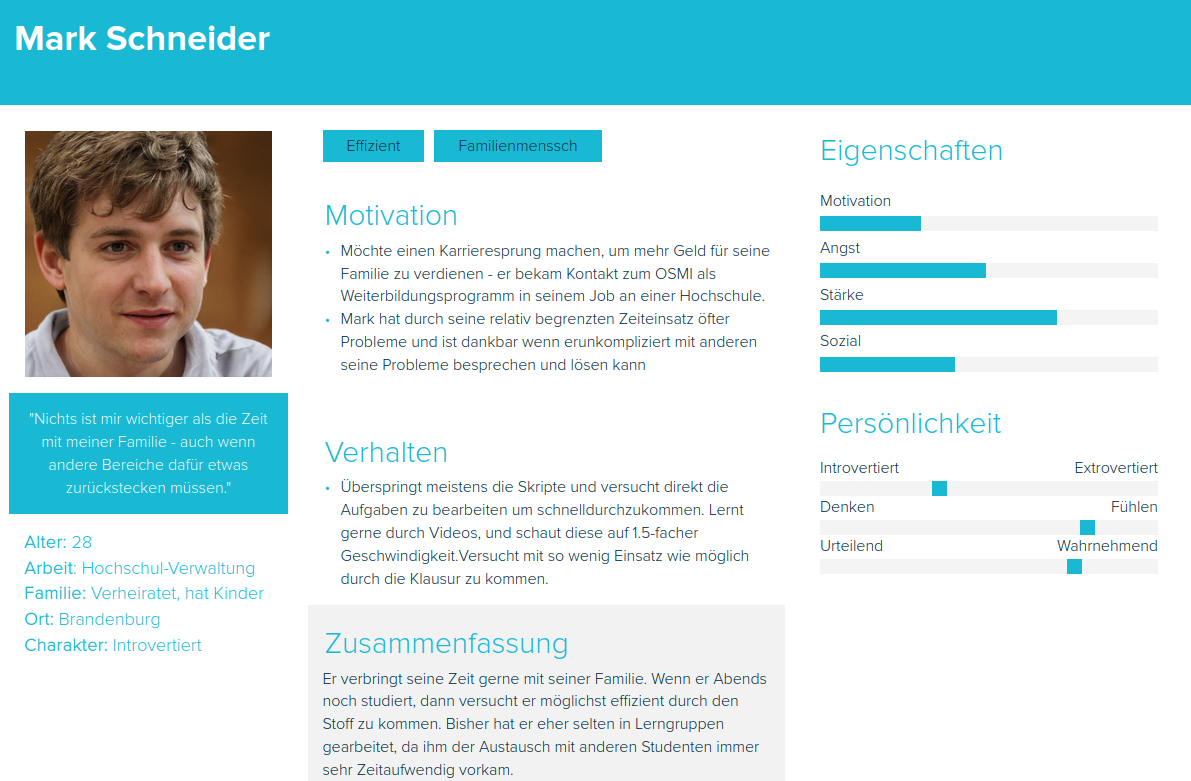
\includepdf[pages=-,landscape]{./images/persona-mark.jpg}

\newpage

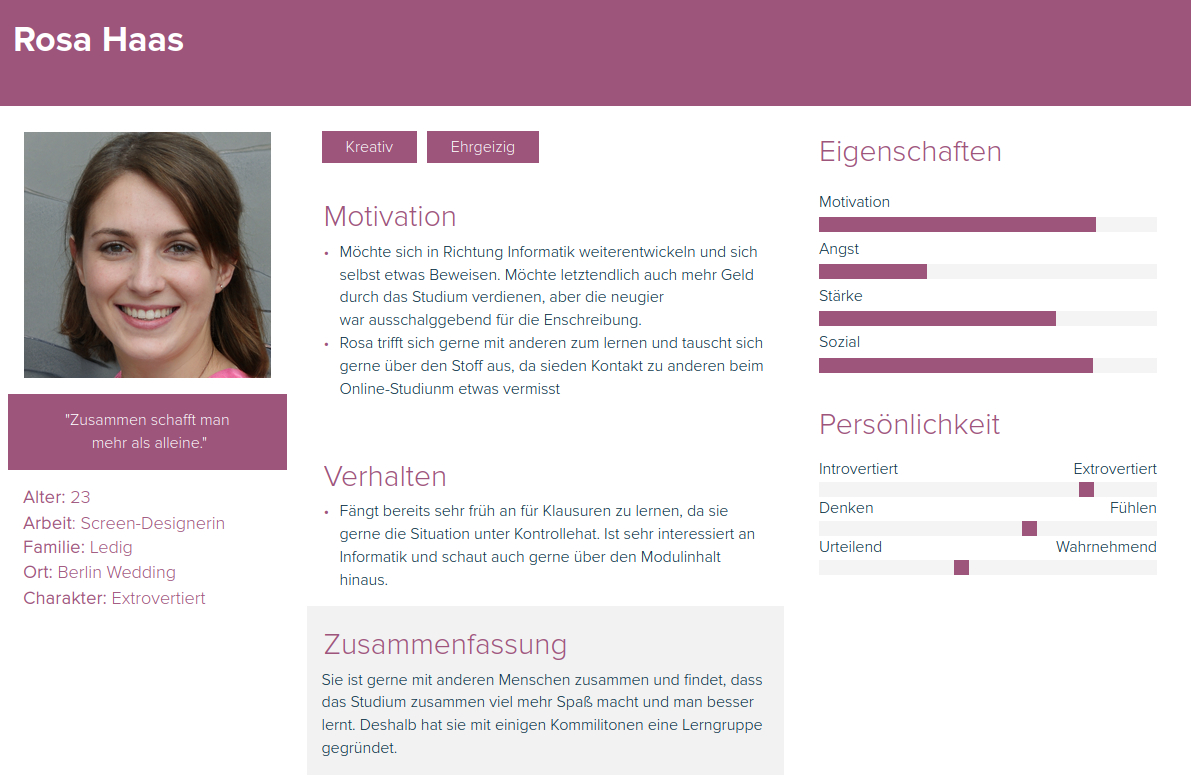
\includepdf[pages=-,landscape]{./images/persona-rosa.jpg}

\newpage

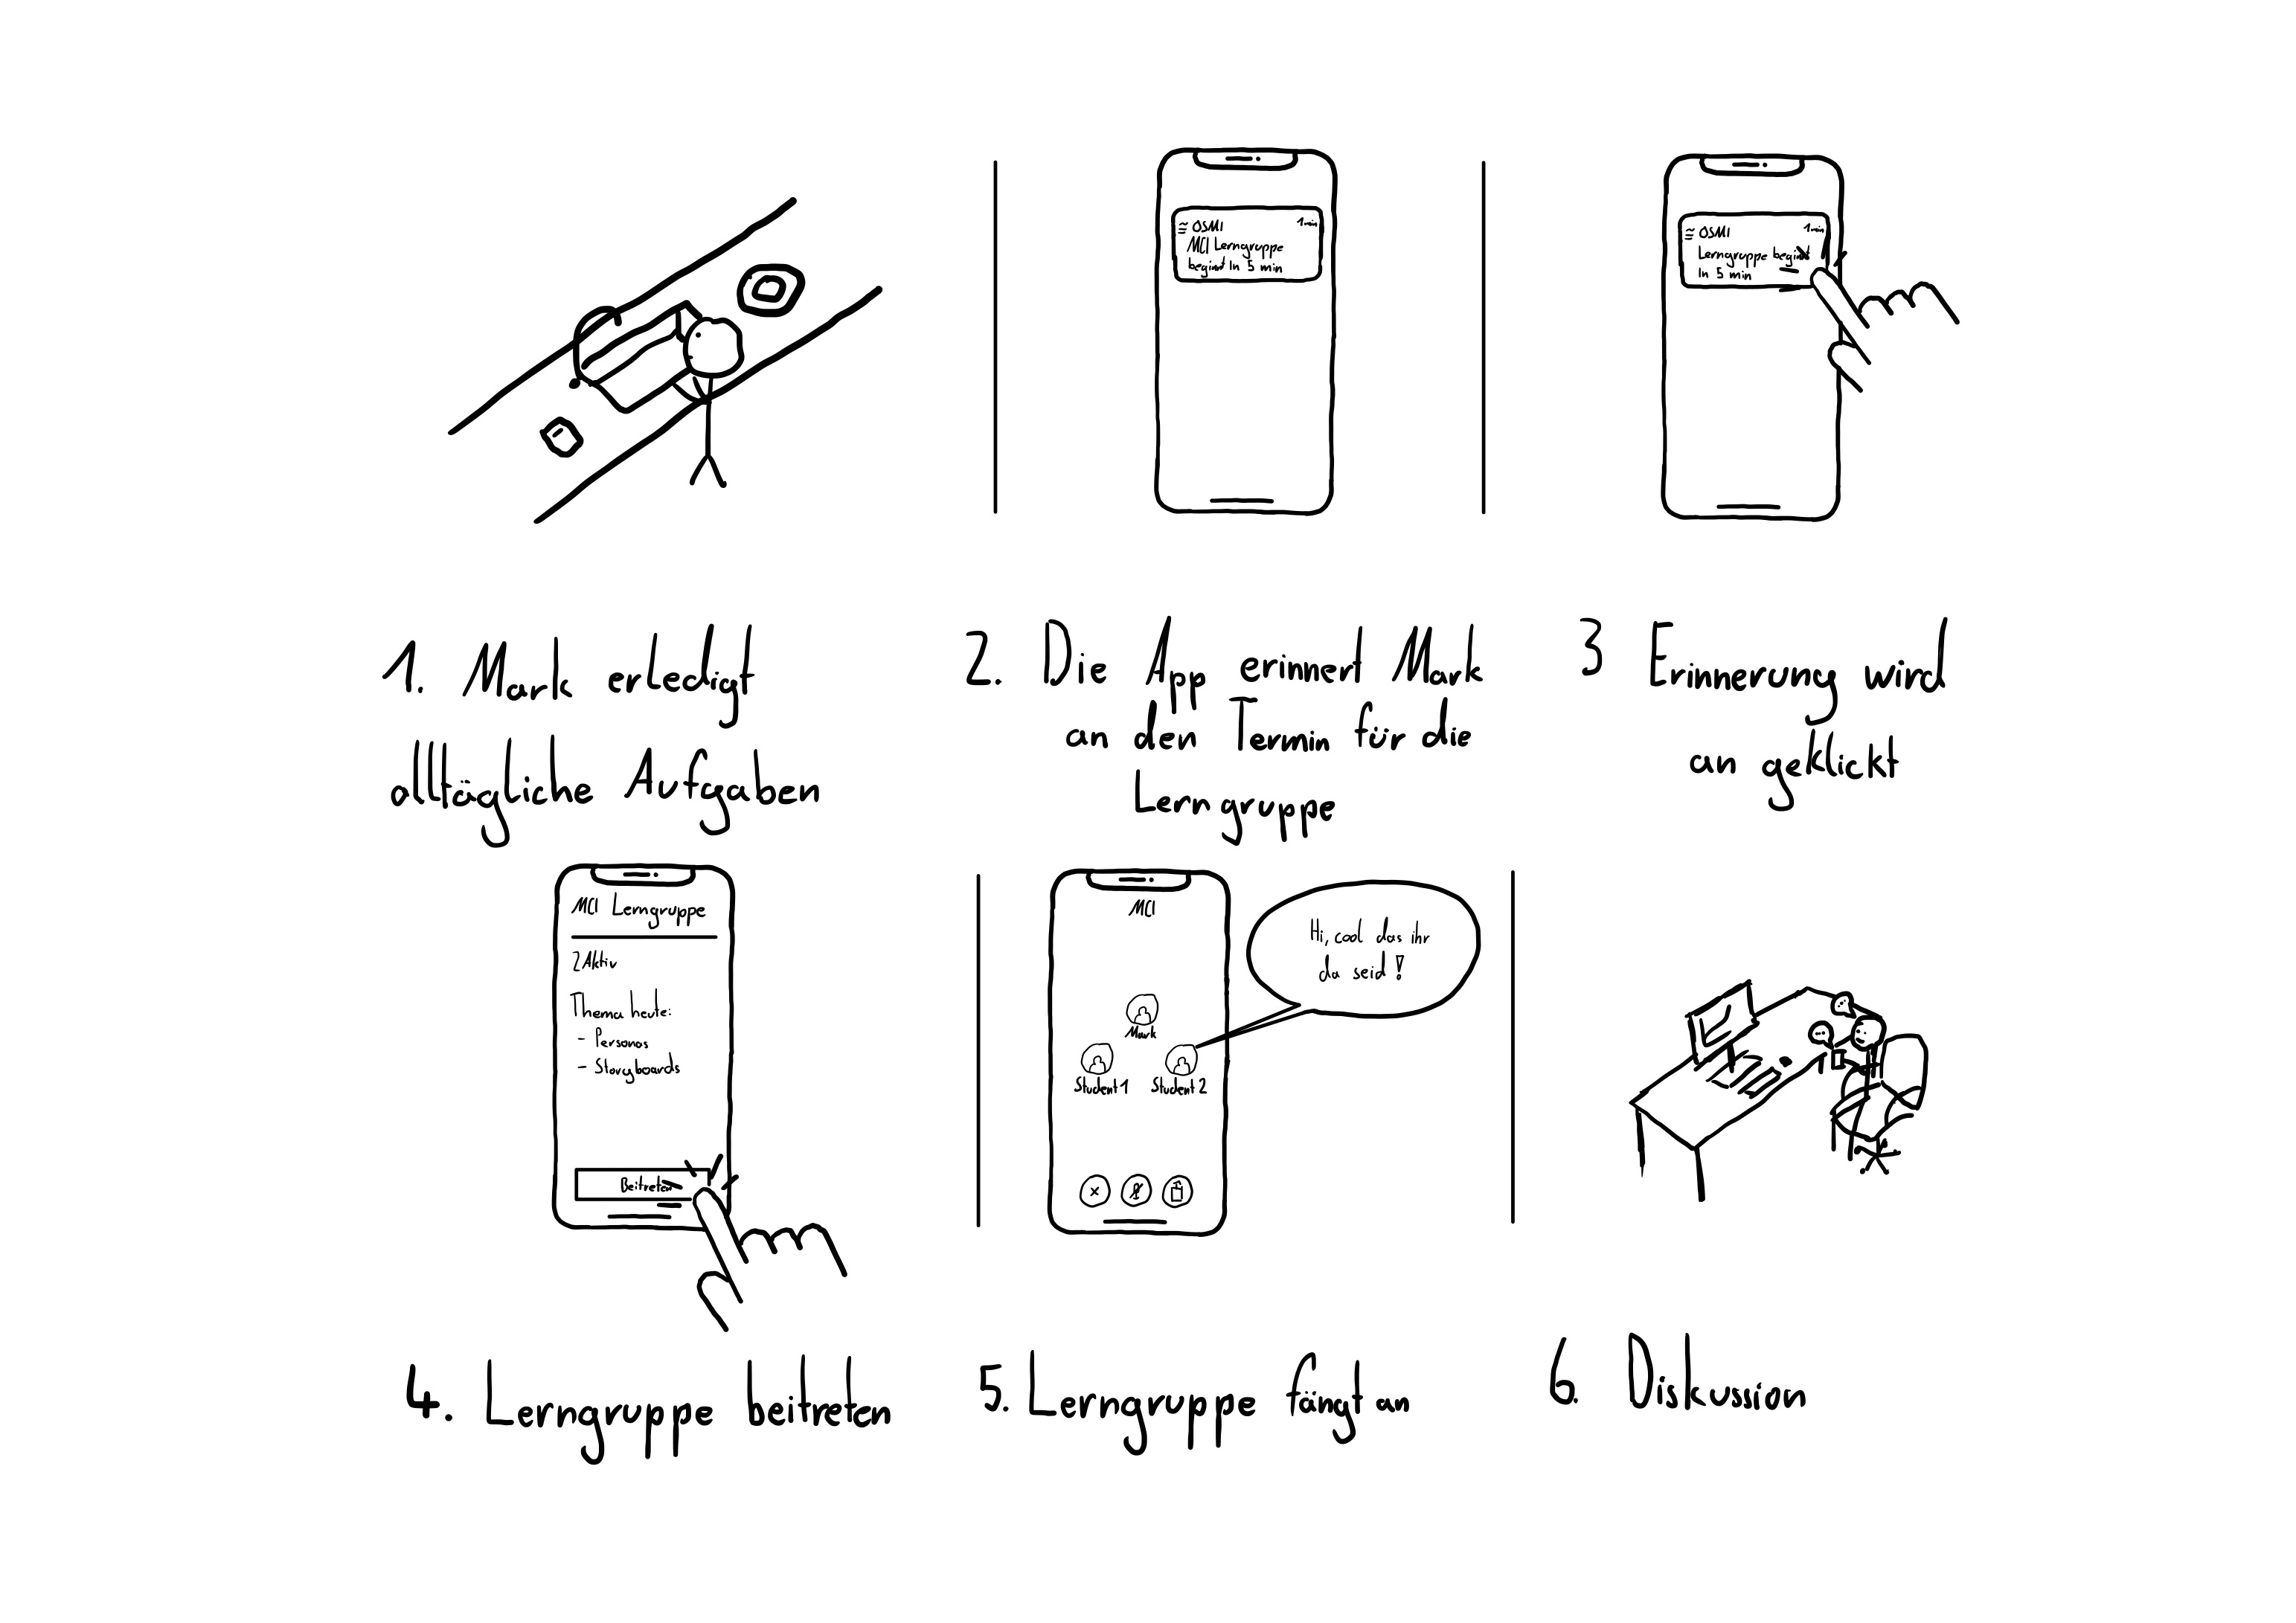
\includepdf[pages=-,landscape]{./images/storyboard-1-mark.jpg}

\newpage

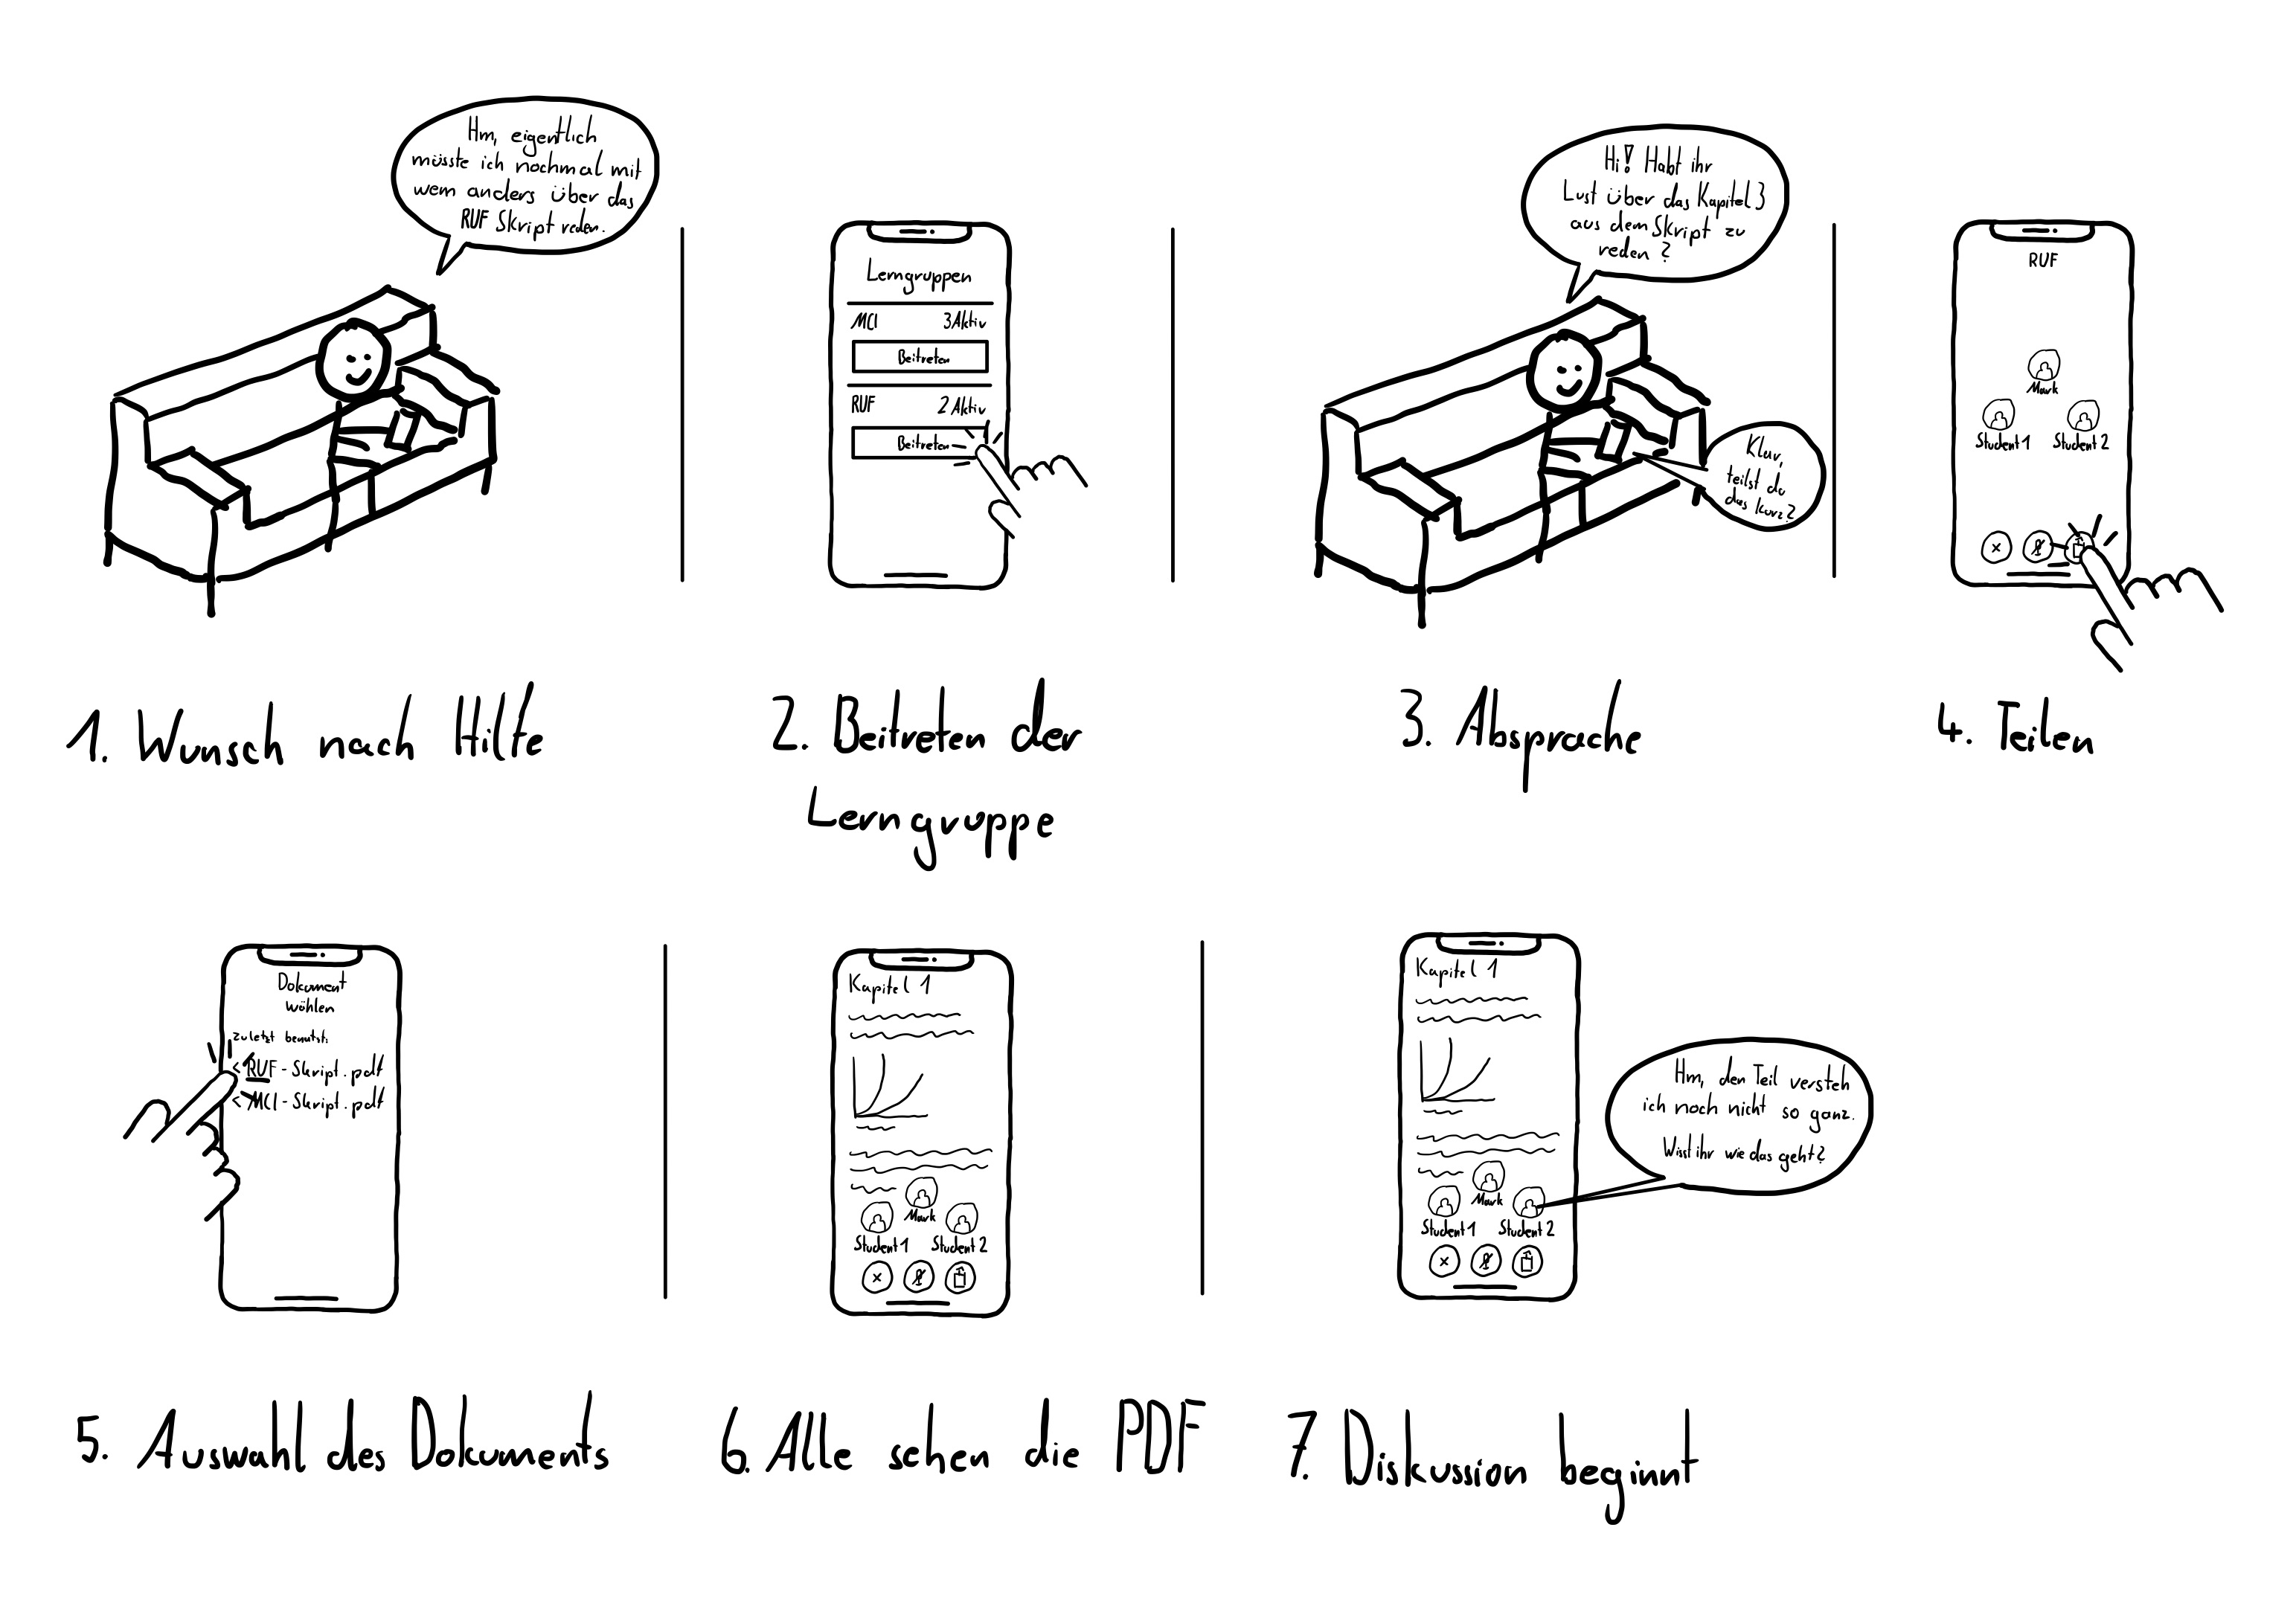
\includepdf[pages=-,landscape]{./images/storyboard-2-mark.jpg}

\newpage

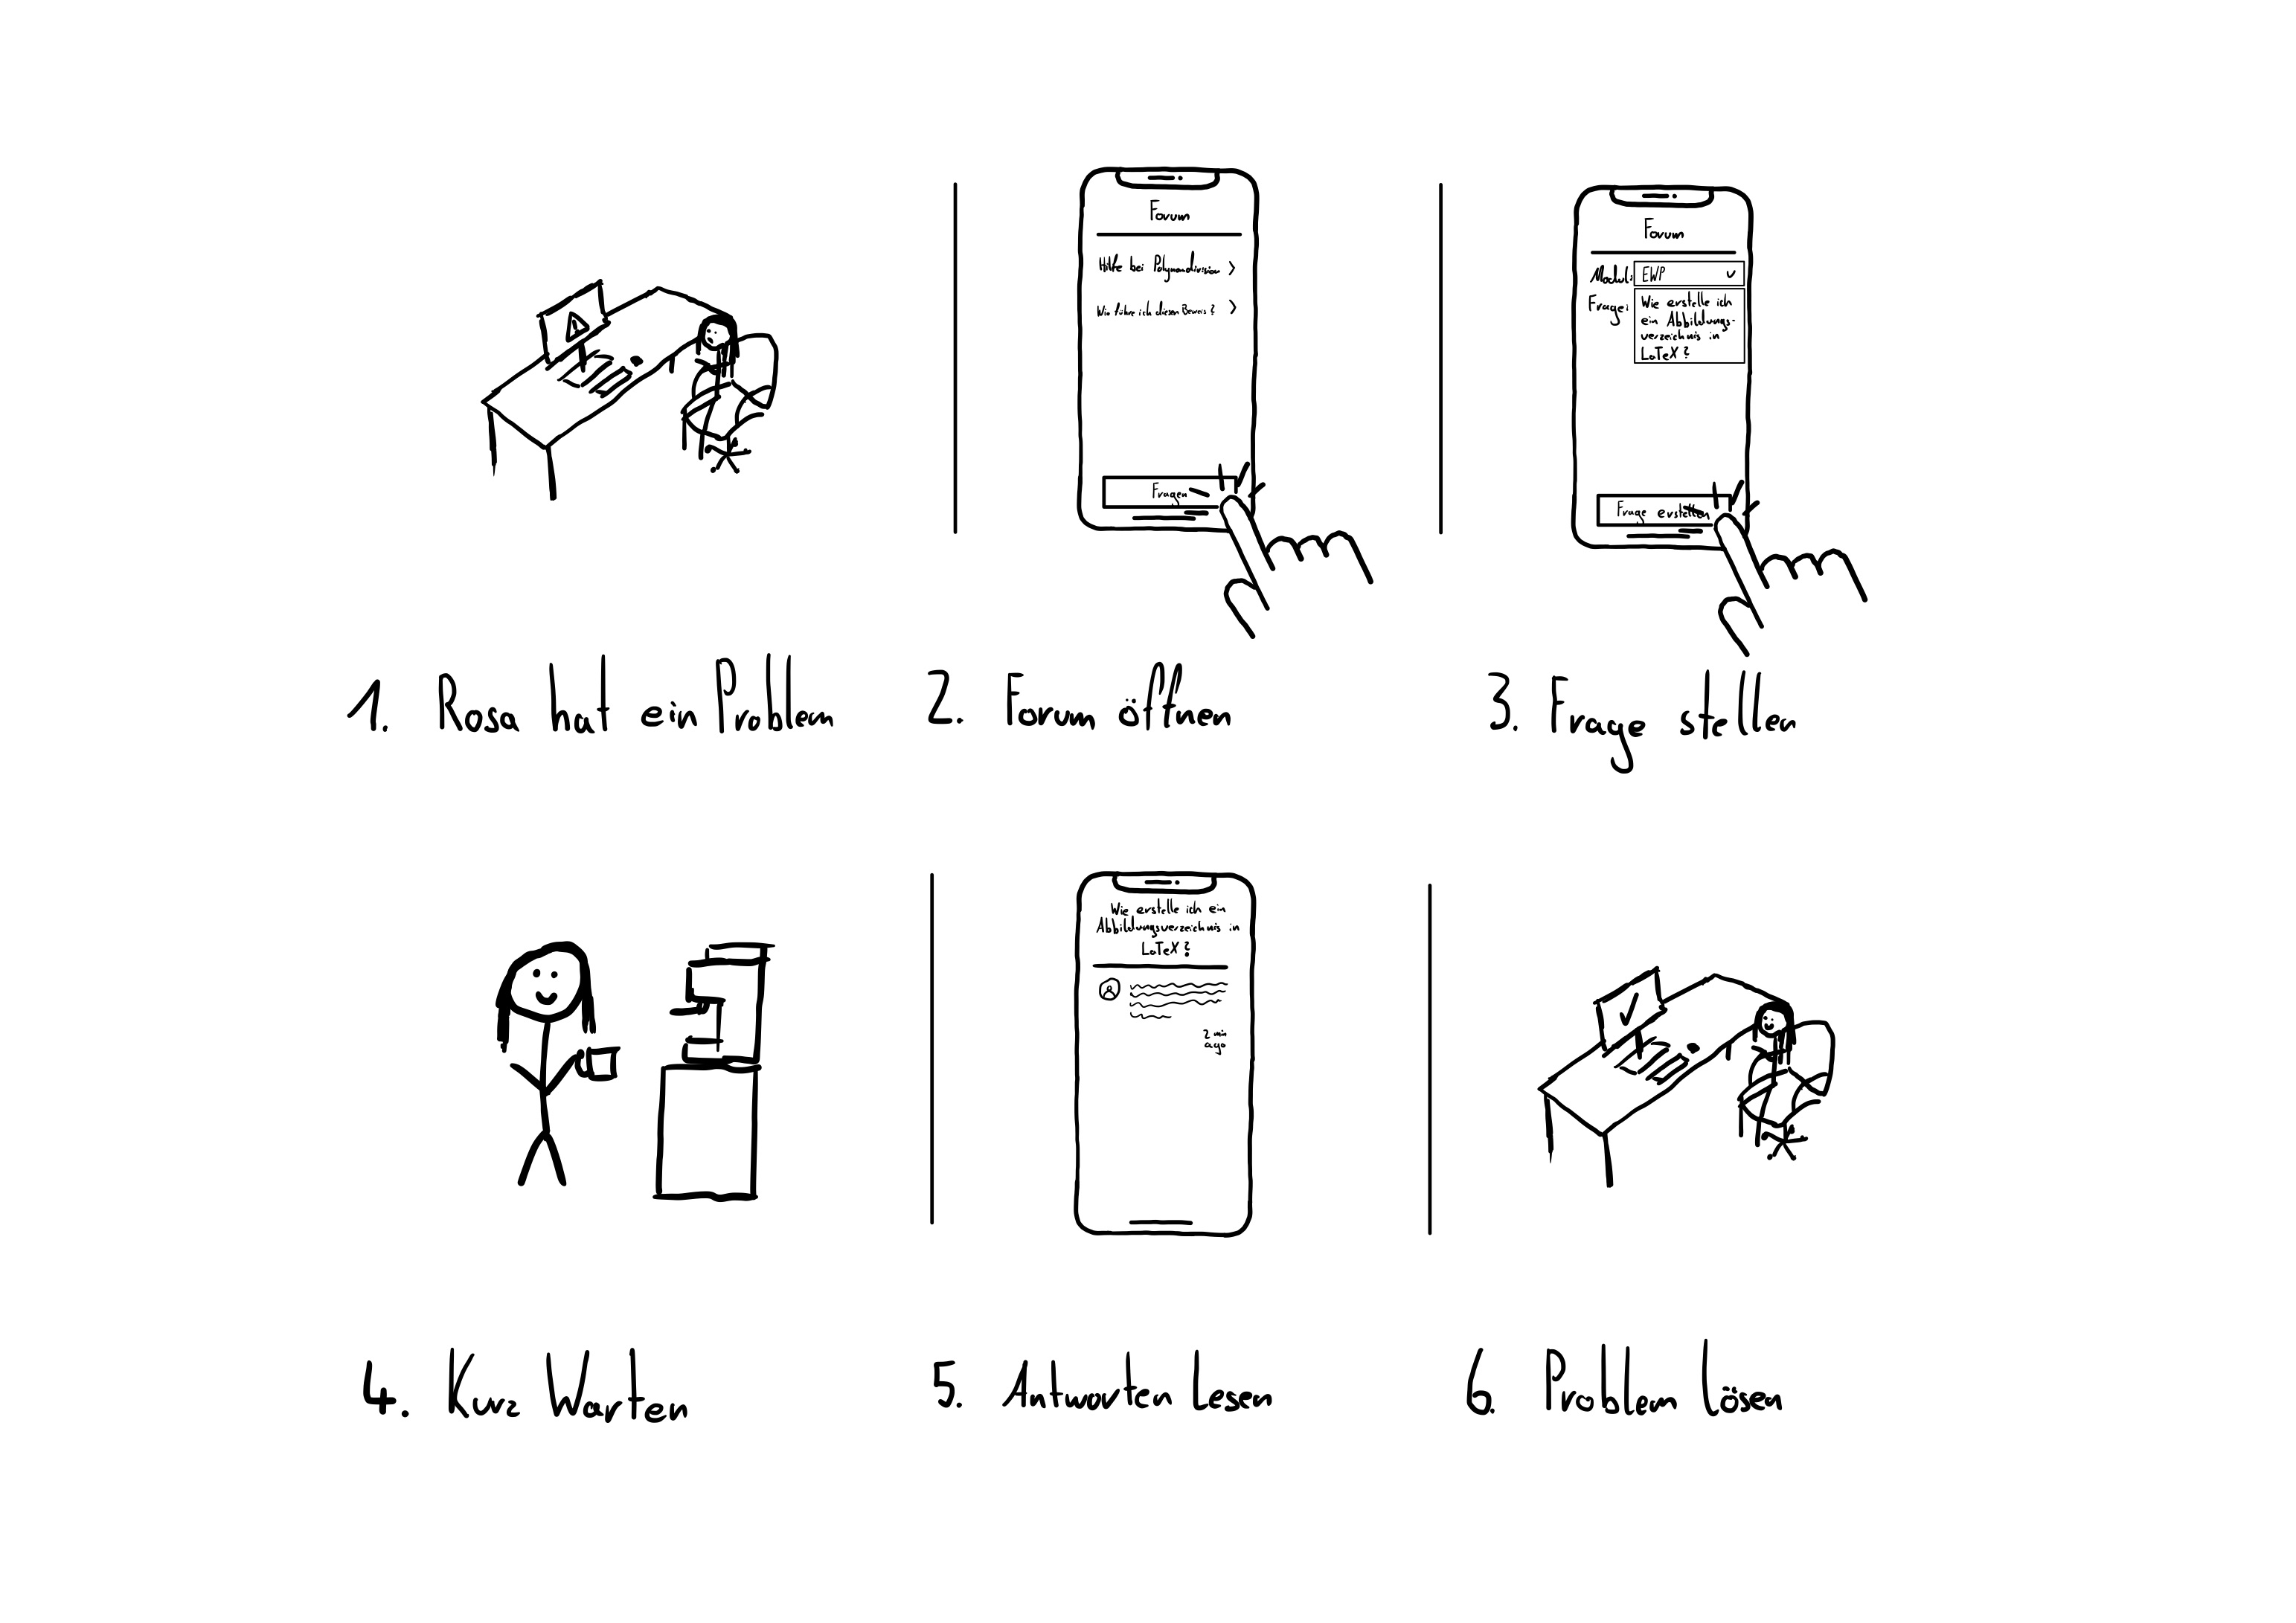
\includepdf[pages=-,landscape]{./images/storyboard-3-rosa.jpg}

\newpage

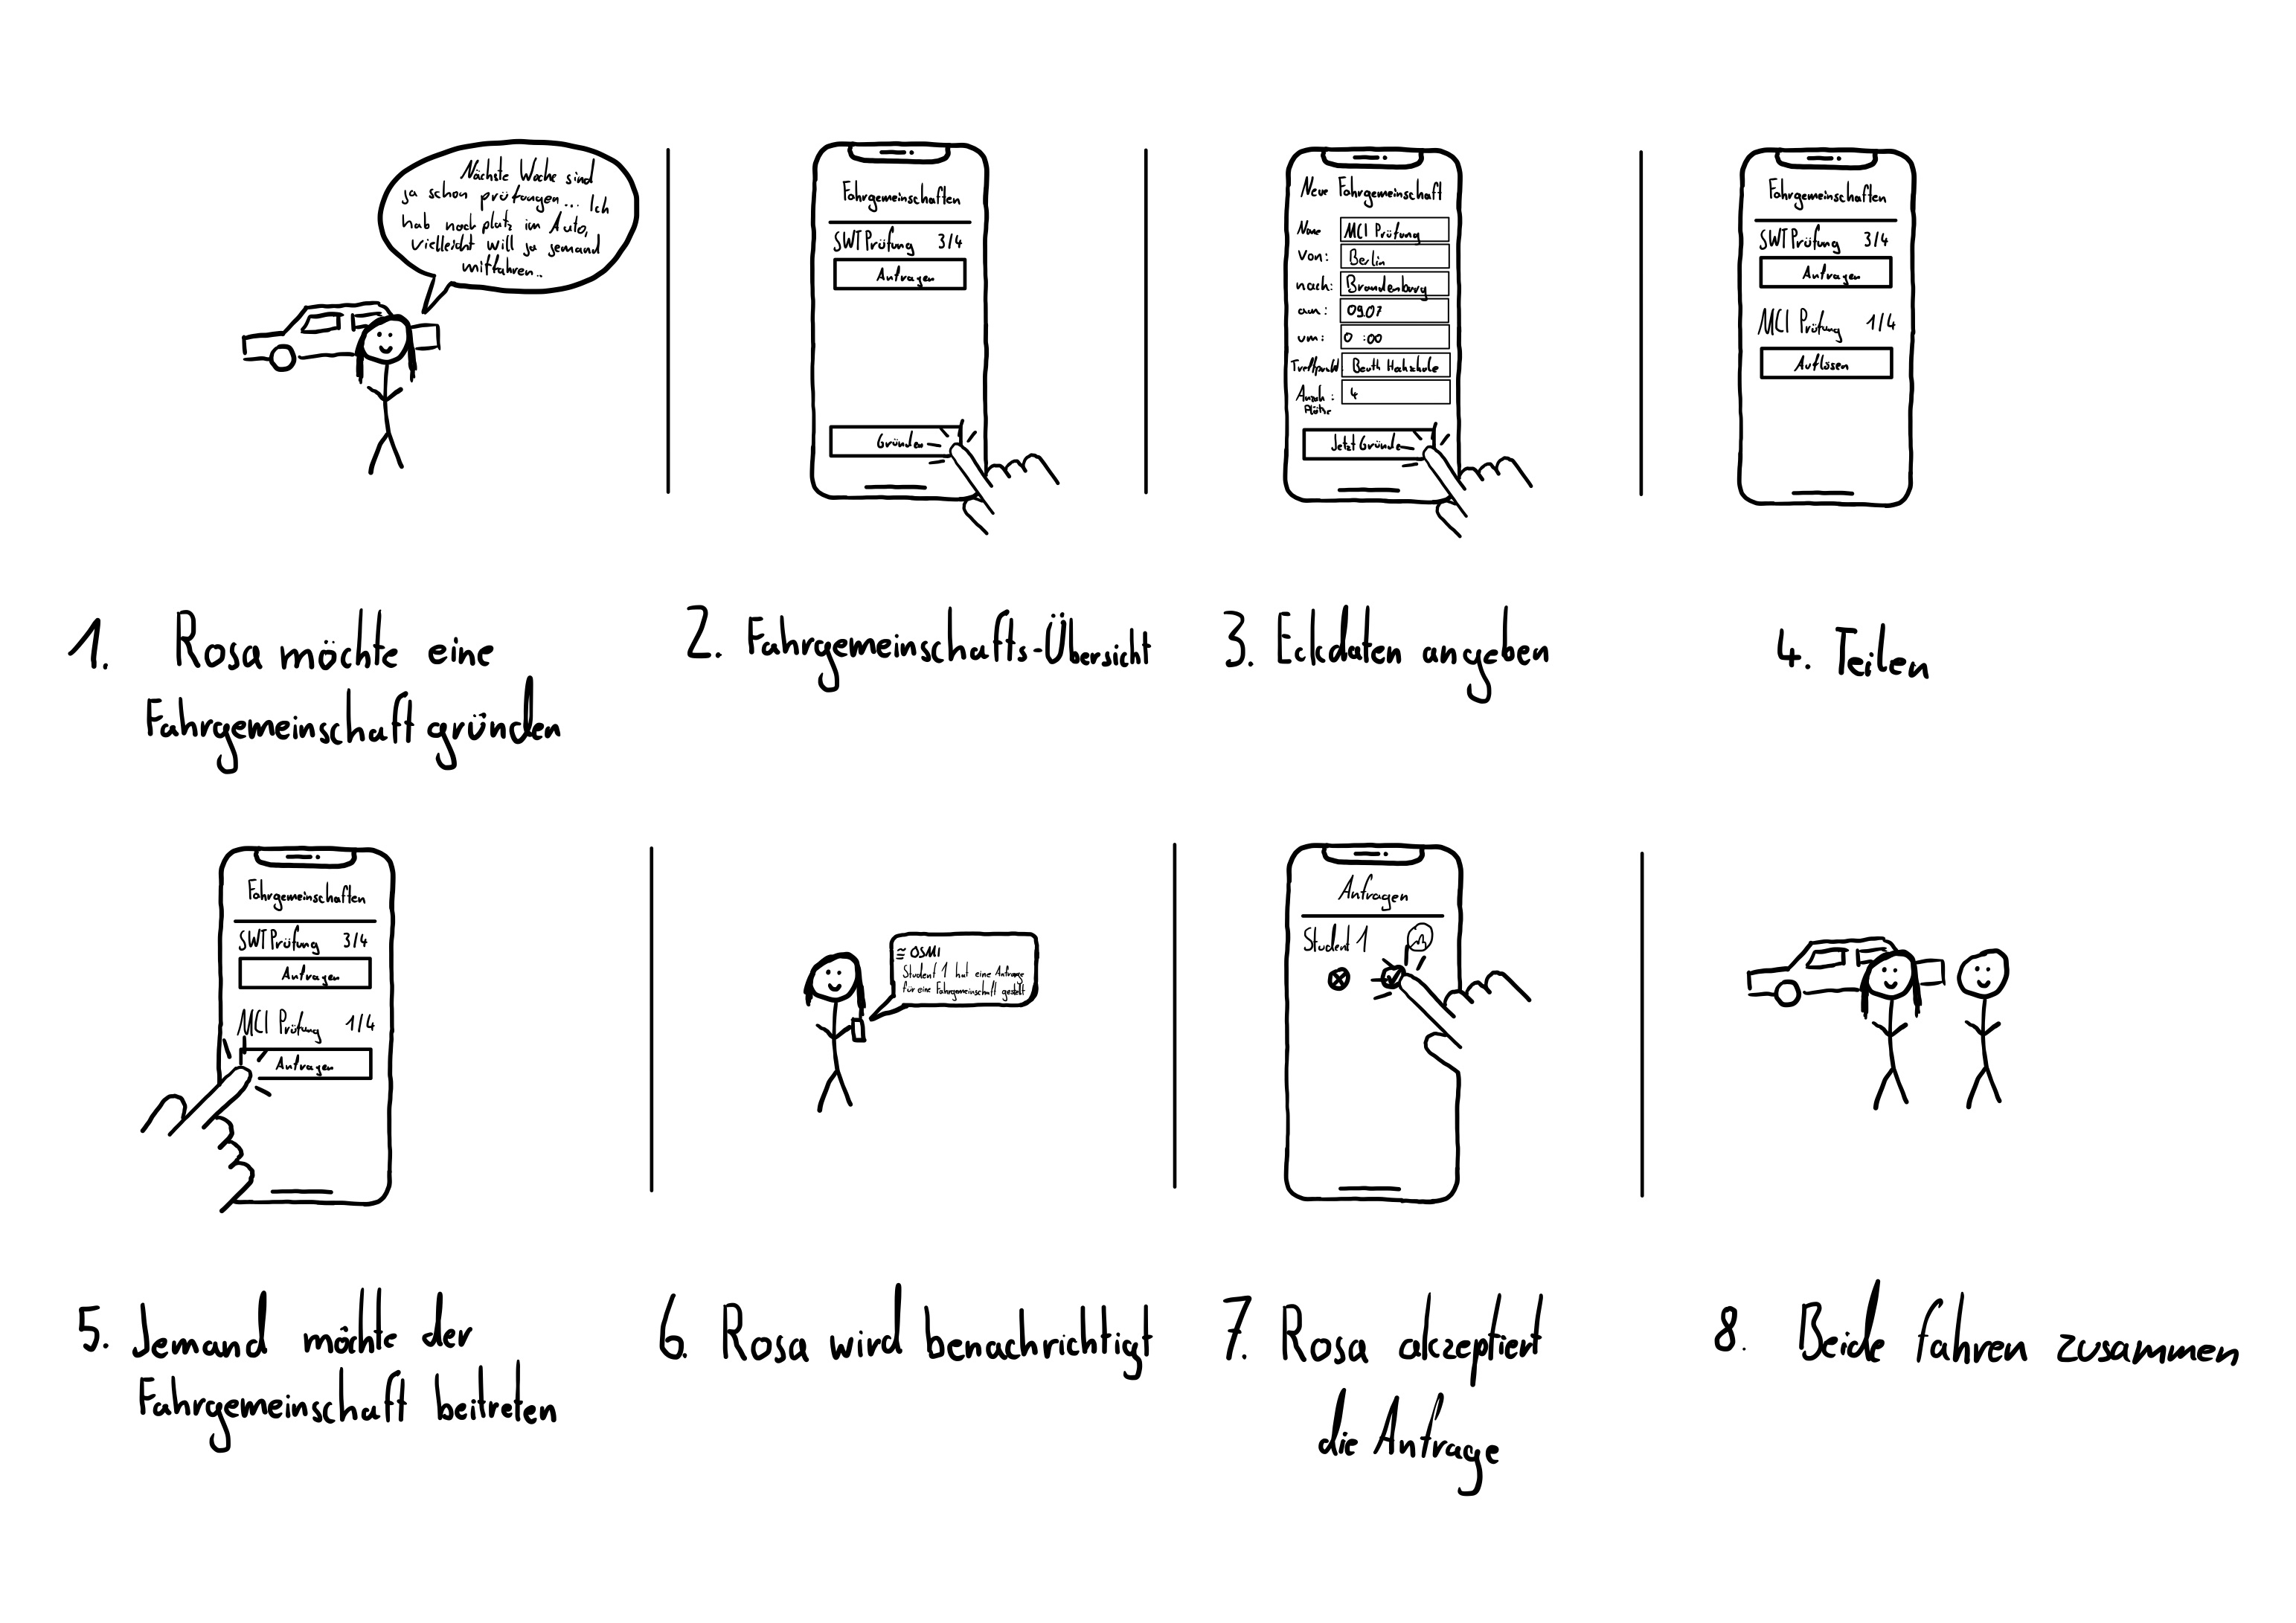
\includepdf[pages=-,landscape]{./images/storyboard-4-rosa.jpg}

\end{document}
